\documentclass{article}
\usepackage{tikz}
\usetikzlibrary{arrows.meta, positioning}

\begin{document}

\section*{Programmfluss -- Übersicht}

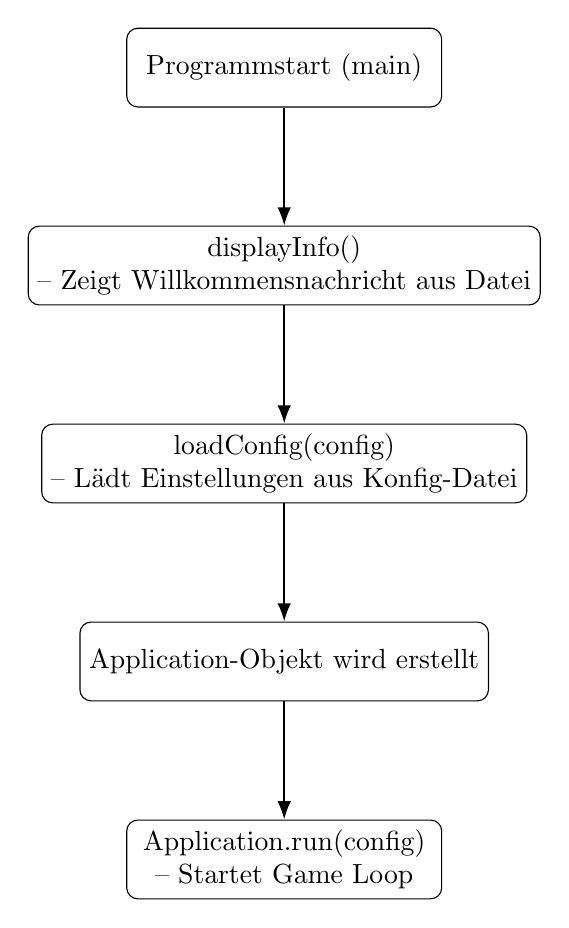
\begin{tikzpicture}[
  node distance=1.5cm and 2.5cm,
  every node/.style={draw, rounded corners, align=center, minimum width=4cm, minimum height=1cm},
  arrow/.style={-{Latex}, thick},
]

% Nodes
\node (start)        {Programmstart (main)};
\node (display)      [below=of start] {displayInfo()\\-- Zeigt Willkommensnachricht aus Datei};
\node (config)       [below=of display] {loadConfig(config)\\-- L\"adt Einstellungen aus Konfig-Datei};
\node (appCreate)    [below=of config] {Application-Objekt wird erstellt};
\node (appRun)       [below=of appCreate] {Application.run(config)\\-- Startet Game Loop};

% Arrows
\draw [arrow] (start)     -- (display);
\draw [arrow] (display)   -- (config);
\draw [arrow] (config)    -- (appCreate);
\draw [arrow] (appCreate) -- (appRun);

\end{tikzpicture}

\end{document}
